\subsection{Kernel Treiber}

\begin{wrapfigure}[23]{o}[1cm]{8cm}
\dirtree{%
.1 /.
.2 install\_driver.sh.
.2 .gitignore.
.2 README.md.
.2 doc/.
.2 app/.
.2 driver/.
.3 Makefile.
.3 spidev\_disabler.dts.
.3 src/.
.4 fanctrl.c.
.4 fanctrl.h.
.4 fops.c.
.4 fops.h.
.4 pwm.c.
.4 pwm.h.
.4 temp.c.
.4 temp.h.
.4 ioctl.c.
.4 ioctl.h.
}
\caption{Ordnerstruktur des Treibers}
\label{fig:driverdirectory}
\end{wrapfigure}

Der Code des Kernel-Treibers ist in \texttt{C99} geschrieben.
Dieser ist Prozessoragnostisch.
Es werden jedoch existierende low-level Treiber zwischen den Prozessorregistern und Kerenlspace erwartet, die die Kommunikation über \gls{i2c} und \gls{spi} abstrahieren.
Das Modul an sich ist lediglich von linux-Headern abhängig.
Der Treiber ist auf verschiedene \texttt{C}-Dateien aufgeteilt.
Die Struktur des Treibers ist in \autoref{fig:driverdirectory} aufgeführt.
Der Tatsächliche Quellcode für den Treiber befindet sich lediglich im \texttt{src} Ordner.
Alle anderen Dateien sind notwendig jedoch kein direkter Teil des Treibers.

Die Haupt-Datei mit dem Anfangspunkt des Treibers ist in \texttt{fanctrl.c}.
Darin wird das Treibermodul initialisiert, registriert, ausgeführt und schließlich auch de-initialisiert.
Der Kernel-Treiber kann über sowohl durch \gls{fops} als auch mit \gls{ioctl} mit dem Userspace kommunizieren.
Dies wird in den \texttt{fops.c} und \texttt{ioctl.c} und deren jehweils dazugehörigen Header-Files implementiert.
Die anderen zwei Hauptfunktionen, die Kommunikation über \gls{i2c} und \gls{spi} werden in \texttt{temp.c} und \texttt{pwm.c} respektiv implementiert.
In den folgenden Abschnitten werden die implementierten Funktionen, zusätzliche Dateien und der Kompilierungs/Installationsvorgang beschreiben.

\subsubsection{Temperatursensor über \acrshort{i2c}}

Der Temperatursensor ist in \texttt{./src/temp.c} und \texttt{./src/temp.h} implementiert.
Mit der Funktion \texttt{tempInit} wird der \gls{i2c} Adapter initialisiert.
Dannach wird ein neuer \gls{i2c} Device struct hinzugefügt und der Treiber wird dem Adapter registriert.
Der Device beinhält die Informationen über Device Name und Addresse.
Ist der Adapter initialisiert wird dieser mit \texttt{tempDeinit}zum Programm Ende, falls er erfolgreich initialisiert wurde, wieder deinitialisiert.
Dabei werden alle vom \gls{i2c} Adapter genutzen Ressourcen für den Treiber frei gegeben.
Auf dem \gls{rpi} muss \gls{i2c} durch die \texttt{raspi-config} aktiviert werden.

Der \texttt{TMP102} Sensor gibt Messdaten mit 13-Bit Präzision bei einer Auflösung von $0.0625\si{\degree C}$ am \gls{lsb} an.
Um einen Messwert zu einer Temperatur zu konvertieren müssen zuerst zwei Byte gelesen werden.
Diese müssen zu einem 16-Bit Wert, welcher den ogrinellen 13-Bit Messwert beinhaltet, konkatiniert werden.
Anschlie{\ss}end muss der Messwert linear abgebildet werden, dass hei{\ss}t mit der Auflösung pro \gls{lsb} multiplizieren.
Die \gls{fpu} sollte unter allen Umständen nicht aus dem Kernelspace verwendet werden,
da die Kontextänderung abträgliche Performanceimplikationen auf Userspace Applikationen mit sich führen kann.
Die berechnung wird folglich mit der Integerdivision des Kehrwerts wie in \autoref{eq:temp-convert} ausgeführt.
Der Fehler der Berechnung wird in \autoref{eq:temp-error} aufgeführt und in \autoref{fig:rounding-err} visualisiert.
Der resultierende Rundungsfehler manifestiert sich als Rauschen.
Da unsere Anwednung sich nominal bei und über Raumtemperatur in Einer-Stellen Präzision agiert sind die resultierenden Fehler vernachlässigbar.
Die Implementation der Kommunikation mit dem Sensor und Wandlung der Daten ist in \autoref{code:i2c-convert} gegeben.

\begin{equation}
    \vartheta = \texttt{M}_D \cdot 0.0625\si{\celsius} = \frac{\texttt{M}_D}{\left(0.0625\si{\celsius}\right)^{-1}} = \frac{\texttt{M}_D}{16\si{\per\celsius}} \approx \left\lfloor\frac{\texttt{M}_D}{16\si{\per\celsius}}\right\rfloor
    \label{eq:temp-convert}
\end{equation}
\begin{equation}
    \begin{aligned}
        \Delta_{\texttt{M}_D} &= \frac{\texttt{M}_D}{16\si{\celsius}} - \left\lfloor\frac{\texttt{M}_D}{16\si{\per\celsius}}\right\rfloor \\[2ex]
        \delta_{\texttt{M}_D} &= \frac{\Delta_{\texttt{M}_D}}{\frac{\texttt{M}_D}{16\si{\celsius}} }\\[2ex]
    \end{aligned}
    \label{eq:temp-error}
\end{equation}

\lstinputlisting[linerange=i2c\ read\ start-i2c\ read\ end, caption={\texttt{./driver/src/temp.c} \gls{i2c} Daten auslesen}, label=code:i2c-convert, float=h]{../../driver/src/temp.c}

\begin{figure}[h]
    \centering
    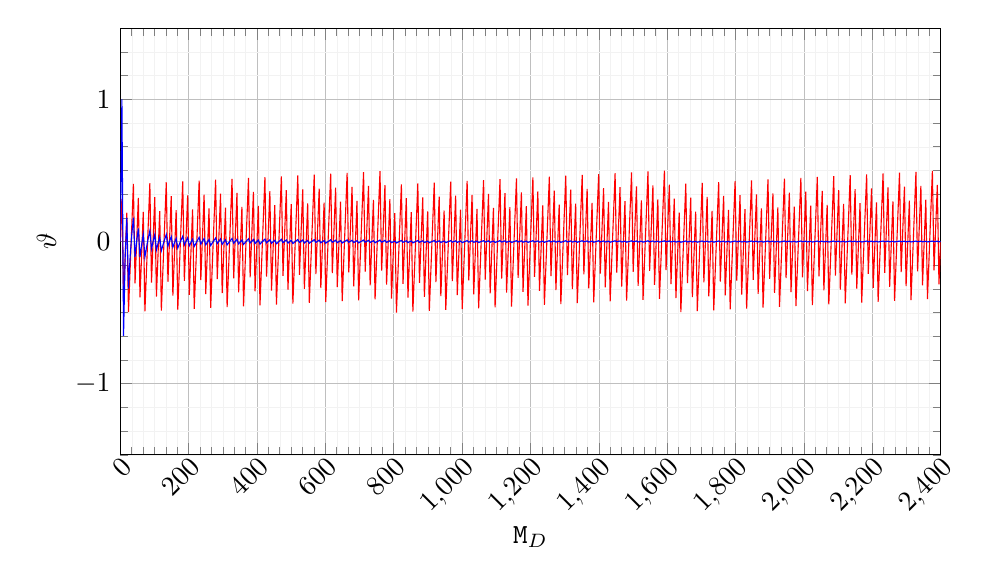
\begin{tikzpicture}
        \begin{axis}[%
            xmin=0,
            xmax=2400,
            ymin=-1.5,
            ymax=1.5,
            samples=500,
            width=12cm,
            height=7cm,
            minor tick num=5,
            grid=both,
            grid style={line width=.1pt, draw=gray!10},
            major grid style={line width=.2pt,draw=gray!50},
            % nodes near coords,
            xlabel near ticks,
            xticklabel style={rotate=45,anchor=north east,inner sep=0mm},
            xlabel={$\texttt{M}_D$},
            ylabel={$\vartheta$},
            ylabel near ticks]
            % \addplot[domain=0:6.4, blue, very thick, smooth, ->] {2.1971*1.8206^x};
            \addplot[domain=0:2400, red] {(x * 0.0625) - round(x / 16)};
            \addplot[domain=0:2400, blue] {((x * 0.0625) - round(x / 16)) / (x * 0.0625)};
        \end{axis}
    \end{tikzpicture}
    \caption[Integerdivisionsinduzierter Rundungsfehler]{Integerdivisionsinduzierter Rundungsfehler der Temperatursensorkonversion aus \autoref{eq:temp-error}.
    \textcolor{red}{Rot: Absoluter Fehler $\Delta_{\texttt{M}_D}$.}
    \textcolor{blue}{Blau: Relativer Fehler $\delta_{\texttt{M}_D}$.}
    }
    \label{fig:rounding-err}
\end{figure}

\subsubsection{Potentiometer über \acrshort{spi}}
\subsubsubsection{\acrshort{spi} Implementation}

Die Initialisierung des \gls{spi} Treibers läuft sehr ähnlich zu der des \gls{i2c} Treibers ab.
Die genaue Implementation ist in \texttt{./src/pwm.c} und \texttt{./src/pwm.h} zu finden.
Es wird zuerst ein \texttt{spi\_board\_info} struct angelegt, welches mit den relevanten Daten des \gls{sbc} gefüllt wird.
Dannach wird mit der Funktion \texttt{spi\_busnum\_to\_master} ein geeignerter Bus Master gesucht.
Diser Master implementiert die Schnittstelle zwischen dem Kernel und der Hardware.
Folgend wird mit \texttt{spi\_new\_device} und schließlich \texttt{spi\_setup} ein \gls{spi} Device angelegt und registriet.
Zu jedem Schritt können Fehler auftreten, welche abgefangen werden.
Die Deinitialisierung ist wieder ähnlich.
Ist der \gls{spi} Device erfolgreich geladen, so wird dieser einfach mit \texttt{spi\_unregister\_device} unregistriert.

Um den Wiederstand des Potentiometers zu setzen, wird die in \autoref{code:spi-write} gezeigte Funktion genutzt.
Darin wird eine \gls{spi} Transaktion aus zwei Bytes erstellt.
Der \texttt{MCP} Chip erwartet zuerst das \textit{Command Byte} in Form von \autoref{tab:command-bits}.
Im Code ist dieses als \texttt{0b00010011} festgelegt.
Dadurch werden beide internen Potentiometer das dannach folgdene Byte annehmen.
Da der Duty Cycle propotional und relativ zu dem Wiederstand ist, kann hier der Wert für das Wiederstandsregister auch als Prozentbereich wie in \autoref{eq:interpret} interpretiert werden.
\begin{equation}
    \left[0_{\text{H}}; FF_{\text{H}}\right] \rightarrow \left[0\%; 100\%\right]
    \label{eq:interpret}
\end{equation}

\lstinputlisting[linerange=spi\ write\ start-spi\ write\ end, caption={\texttt{./driver/src/pwm.c} \gls{spi} Potentiometer setzen}, label=code:spi-write, float=h]{../../driver/src/pwm.c}

\subsubsubsection{Devicetree Overlay}
Auf dem \gls{rpi} muss der \gls{spi} Treiber durch \texttt{raspi-config} aktiviert werden.
Dadurch werden unter \texttt{/dev} zwei \gls{spi} Treiber angelegt und das Hardware \gls{spi} Subsystem aktiviert.
Die angelegten Treiber stellen eine \gls{api}-Verbindung zwischen Kernelspace und der Hardware dar.
Jedoch werden durch die Treiber die \gls{ss} Signale belegt.
Der Treiber zur Kommunikation über \gls{spi} funktioniert, kann jedoch aufgrund dessen nicht durch externe Programme im Kernelspace beansprucht werden.
Um dies zu umgehen muss der Zugriff auf die \gls{ss} Signale durch die durch das System bereitgestellten Treiber unterbunden werden.
Dazu wird der Devicetree zur Laufzeit mit einem Patch injeziert.
Deswegen stehen die \gls{ss} Signale frei zur Verfügung, um durch unseren Treiber aus dem Kernelspace genutzt zu werden.
Das Devicetree Overlay wird mit dem devicetree compiler kompiliert:
\begin{lstlisting}[language=bash, numbers=none]
dtc spidev_disabler.dts -O dtb > spidev_disabler.dtbo
\end{lstlisting}
\noindent
Das generierte Overlay wird dannach injeziert:
\begin{lstlisting}[language=bash, numbers=none]
sudo dtoverlay -d . spidev_disabler
\end{lstlisting}

\subsubsection{\acrshort{fops}}

Die \gls{fops} Operationen werden in \texttt{./src/fops.c} und \texttt{./src/fops.h} implementiert und in \texttt{./src/fanctrl.c} im \texttt{file\_operations} struct registriert.
Der \gls{fops} Treiber legt eine Pseudodatei unter \texttt{/etc/fanctrl} an.
Durch lesen der Datei wird der Sensor kontinuierlich ausgelsen und der Temperaturwert ausgegeben.
Durch schreiben in die Datei wird der Duty Cycle gesetzt.
Dieser muss im Intervall zwischen $\left[0_{\text{H}}; FF_{\text{H}}\right]$ liegen.

\subsubsection{\Acrshort{ioctl}}

Die \gls{ioctl} Treiber werden in \texttt{./src/ioctl.c} und \texttt{./src/ioctl.h} implementiert und auch in \texttt{./src/fanctrl.c} im \texttt{file\_operations} struct registriert.
Der Header definiert zwei \gls{ioctl} Kommandos.
Diese sind in \autoref{tab:ioctl} aufgeführt.
Die Implementation findet in der dazugehörigen C-Datei in \texttt{dev\_ioctl} statt.
Durch \texttt{CMD\_READ\_TEMP} wird die Temperatur gelesen und zurückgegeben.
Mit \texttt{CMD\_SET\_SPEED} wird der duty cycle zu dem Übergabeparameter gesetzt.

\begin{table}[h]
    \centering
    \begin{tabular}{|l|l|l|l|l|}
        \hline
        \textbf{IOCTL Name} & \textbf{Richtung} & \textbf{Typ} & \textbf{Nr} & \textbf{Größe} \\
        \hline
        \hline
        \texttt{CMD\_READ\_TEMP} & Read & '\texttt{A}' & $01_{\text{H}}$ & \texttt{u32} \\
        \hline
        \texttt{CMD\_SET\_SPEED} & Write & '\texttt{A}' & $02_{\text{H}}$ & \texttt{u32} \\
        \hline
    \end{tabular}
    \caption{Verfügbare \acrshort{ioctl} Kommandos}
    \label{tab:ioctl}
\end{table}

\subsubsection{Kompilierung und Verlinkung}

Der Treiber kann automatisch mit dem \texttt{Makefile} kompiliert und als Kernel Objekt verlinkt werden.
Danach kann das erstelle Kernel Objekt auch in den Kernel geladen werden.
Um den Entwicklungslebenszyklus zu vereinfachen besteht auch die Möglichkeit den gesamten Zyklus automatisch auszuführen.
Mit dem \texttt{./install\_driver.sh} Skript wird das Kernelmodul entladen, neu kompiliert, das Devicetree Overlay neu geladen und das Kernel Modul wieder neu geladen.
